\newpage
\part{Evolution}
\subsection*{Forklar hvad der forstås ved evolution. Kom herunder ind på, hvad der driver evolution}
Evolution er de processer, hvormed livet på jorden har udviklet sig over tid. Det er også en central del af biologi og hjælper med at forklare livsformer og de forskelle, vi ser mellem dem. Evolution drives af en mekanisme kendt som naturlig udvælgelse. Naturlig udvælgelse er en proces, hvor organismer med egenskaber, der er gunstige for deres overlevelse og reproduktion, har større sandsynlighed for at overleve og formere sig. 
\begin{figure}
    \centering
    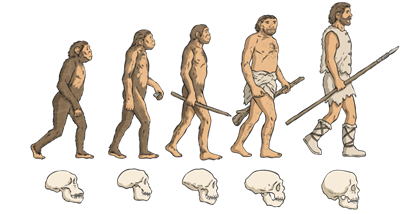
\includegraphics[width=0.8\textwidth]{figurs/Picture3.png}
    \caption{Evolution}
    \label{fig:evolution}
\end{figure}
\subsection*{Redegør for mutationer, samt hvordan de kan lede til variation. Inddrag gerne øvelse om selektion.}
Mutationer er ændring af cellers DNA. Mutationer sker gennem hele cellens levetid og kan have mange konsekvenser. 

Dna er et makromolekyle med mange informationer, derfor når det skal kopieres og deles ved celledelingerne, kan der opstå fejl på grund af radioaktiv stråling, solskoldninger, eller kemiske stoffer, der ødelægger de kemiske bindinger i molekylerne. Når informationerne skades, vil resultatet ofte blive, at de proteiner DNA'et koder for, mister dens funktion. 
\subsection*{Med udgangspunkt i øvelsen om dykkerrefleks, ønskes en diskussion af udvikling af mekanismen, samt en diskussion om udviklingen af nye arter.}
I mennesker har vi en refleks som sidder i næsten, den refleks er meget følsom over for kulde. Hvis den refleks mærker at det bliver koldere sender det et signal til hjernen for at advare om at kroppen muligvis er ved at drukne. Derefter bliver pulsen sænket for at reducere mængden af ilt der bliver brugt i kroppen som gør at man kan overleve lidt længere tid. Et sted hvor dykkerrefleksen bliver brugt meget er hos dyr som hvaler, delfiner, pingviner og sæler da de ikke har gæller til at trække vejret under vandet men kan stadigvæk være under vandet i længere perioder. 